
\section{Introduction}
\label{sec:introduction}

Real-time collaborative editors allow authors to simultaneously write
shared documents~\cite{greenberg1994real}. Trending editors such as
Google Docs rely on central servers. They raise privacy issues since
service providers take advantage of their mediating position to
observe all users and documents. They also raise scalability issues: a
server is required to support one editing session, so handling many
editing sessions require many ressources. Also managing many
participants in one editing session is costly and may overload the server.

\CRATE is a distributed and decentralized
\textsc{c}ollabo\textsc{rat}ive \textsc{e}ditor providing scalable
real-time editing capabilities directly within existing web
browsers. Compared to state of art, \CRATE is the first real-time
editor that only require browsers to support collaborative editing and
handle transparently small groups to large groups of
users. Consequently, \CRATE is not restricted to traditional
collaborative editing but can also be used in massive online lectures,
TV shows or large conferences to allow users to share their
notes. 

Suppose a massive online lecture platfrom allows participants to share
notes about the lecture. Many lectures can run in parallel with
various number of participants ie. from few to thousands. Even during
one editing session, the number of participants can change
significantly, from thousands to few hundreds. The size of document
produced by users is also hard to predict: it can vary from few pages
to hundreds of pages. Building a decentralized editor able to handle
all these situations require to combine different algorithms to
achieve an acceptable trade-off between space, time and communication
complexities.

To provide availability and responsiveness, \CRATE is based on the
optimistic replication scheme~\cite{saito2005optimistic}. Thus, each
editor replicates the document locally and directly performs
operations on it. Next, changes are spread to all other
participants. When the same set of operations are applied by editors,
the replicates converge to an equivalent state allowing users to read
the same document.  This property is called \emph{strong eventual
  consistency}~\cite{bailis2013eventual}.

\CRATE uses a Conflict\--Free Replicated Data structure (CRDT) for
sequences to ensure strong eventual consistency on the
document~\cite{shapiro2011comprehensive}. Consistency is ensured at
the price of unique identifier attached to each element of the
sequence. Recently, \LSEQ~\cite{nedelec2013lseq} proposed a strategy
to bound the space complexity of these identifiers to $log(n)^2$ where
$n$ is the total size of document. This results avoids to run costly
distributed garbage-collection-like mechanism to maintain the
efficiency of the editor.

Strong consistency is ensured if every operations sent by a user is
eventually received by all participants of the editing
sessions. \CRATE builds an editing session using
\SPRAY~\cite{nedelec2015spray}, a random peer sampling
protocol~\cite{jelasity2007gossip} (RPS) built on top of WebRTC. A
peer-sampling protocol allow participants of a network to just have a
random partial view of whole network. Maintaining this partial view
random ensures the connectivity of the network. Unlike prior RPS,
\SPRAY allow to adapt the size of the partial view to the editing
session size without measuring the number of participants. Since the
propagation protocol of messages~\cite{birman1999bimodal} extensively
uses these tables, the network traffic inherits from this
scalability. Consequently, \CRATE adapts its operation to the need of
the editing session size.

In this paper:
\begin{inparaenum}[(i)]
\item we describe the usage, the architecture and the properties of
  the \CRATE decentralized real-time editor;
\item we describe the setup of a live demo where WWW2016 participants
  join an editing session. We aim to collect a real-world editing
  corpus to validate results obtained in lab. We already run \CRATE on
  Grid'5000 involving up to 600 artificial editors typing.
\end{inparaenum}

Section~\ref{sec:architecture} details the overall architecture of \CRATE along
with its basic functioning. Section~\ref{sec:structure} describes the
distributed data structure that represents the
document. Section~\ref{sec:network} details the network building
operation. Section~\ref{sec:live} states the live experiment setup we
propose. Section~\ref{sec:conclusion} concludes.

\begin{figure*}
  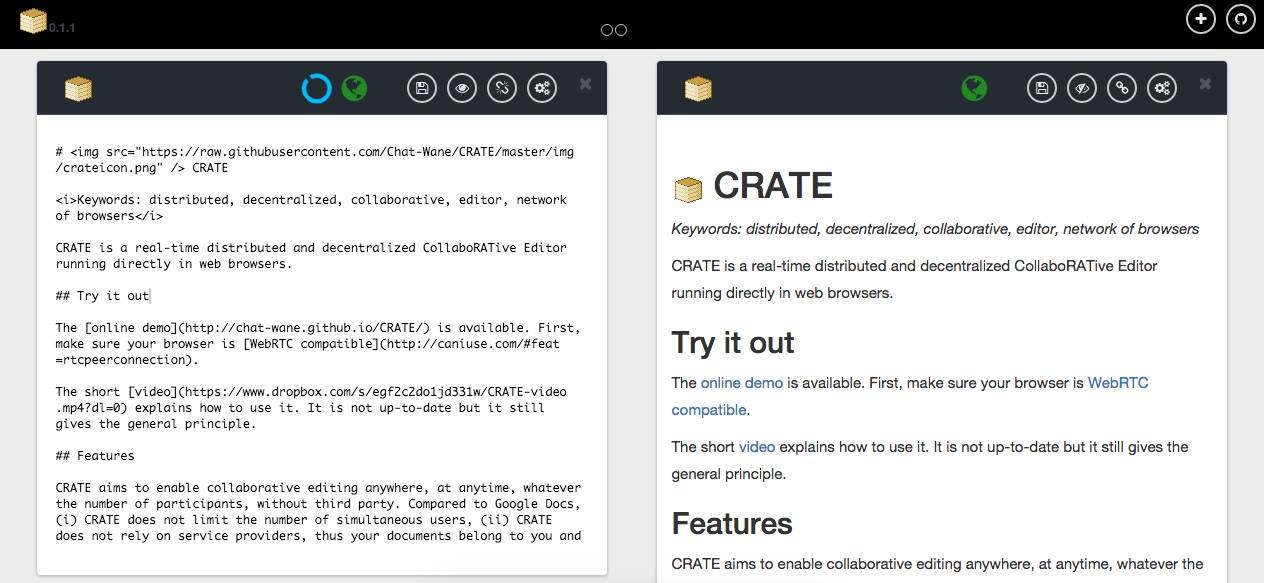
\includegraphics[width=\textwidth]{./img/screenshot.png}
  \caption{\label{img:screenshot} Screenshot of the web application containing
    two editors: on the left, a document is written in markdown language which
    is previewed on the right editor.}
\end{figure*}

%%% Local Variables:
%%% mode: latex
%%% TeX-master: "../paper"
%%% End:
